\epigraph{``Since Newton, mankind has come to realise that the law of physics are always expressed in the language of differential equations"}{Steven Strogatz}

\section{RNN}
\subsection{Introduction}
Weather forecasting has traditionally been done by physical models of the atmosphere, which are unstable to perturbations, and thus are inaccurate for large periods of time\cite{why_rnn}. Since machine learning techniques are more robust to perturbations, it would be logical to combine a neural network with a physical model. Weather forecasting is a sequential data problem, therefore, a recurrent neural network is the most suitable option for this task. 

\begin{definition}
A recurrent neural network is a class of artificial neural networks where connections between nodes form a directed graph along a temporal sequence.
\end{definition}

Before, we delve into the specific example of using a recurrent neural network to predict the future state of the atmosphere, it is necessary to review what a recurrent neural network is. Recurrent Neural Networks (RNNs) are neural networks that are used in situations where data is presented in a sequence. For example, let's say you want to predict the future position of a fast-moving ball. Without information on the previous position of the ball, it is only possible to make an inaccurate guess. If you had, however, a large number of snapshots of the previous position, you are then able to predict the future position of the ball with some certainty. RNNs excel at modelling sequential data such as this. This is due to sequential memory.

In order to intuitively understand sequential memory, the prime example would be the alphabet. While it is easy to say the alphabet from A-Z, it is much harder to go from Z-A. There is a logical reason why this is difficult. As a child, you learn the alphabet in a sequence. Sequential memory is a mechanism that makes it easier for your brain to recognise sequence patterns.

In a traditional neural network, there is an input layer, hidden layer, and an output layer. In a recurrent neural network, a loop is added to pass information forward as seen in the diagram below (provided by Towards Data Science)\cite{intro_rnn}:

\begin{figure}[H]
    \centering
    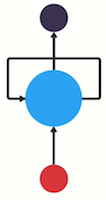
\includegraphics[width=.2\linewidth]{Images/rnn.png}
    \caption{Visualisation of a Recurrent Neural Network}
\end{figure}

The information that is forwarded is the hidden layer, which is a representation of previous inputs. How this works in practise is that you initialise your network layers and the initial hidden state. The shape and dimension of the hidden state will be dependent on the shape and dimension of your recurrent neural network. Then you loop through your inputs, pass the relevant parameter and hidden state into the RNN. The RNN returns the output and a modified hidden state. Last you pass the output to the output layer, and it returns a prediction. 

There is, however, a major problem known as short-term memory. Short-term memory is caused by something known as the vanishing gradient problem, which is also prevalent in other neural network architectures. As the RNN processes more steps, it has troubles retaining information from previous steps. Short-Term memory and the vanishing gradient is due to the nature of back-propagation. This can be comprehended through understanding how a neural network is trained\cite{intro_rnn}.

\begin{definition}
Back-propagation is an algorithm used to train and optimise neural networks.
\end{definition}

To train a recurrent neural network, you use an application of back-propagation called back-propagation through time. Training a neural network has three major steps. First, the relevant data vector is normalised between 0 and 1, the vector is fed into the RNN, and it goes through an activation function. The activation function utilised in the software is the rectified linear activation function\cite{lstm_rnn}. 

\begin{definition}
The rectified linear activation function is a piece-wise linear function that will output the input directly if is positive, otherwise, it will output zero.
\end{definition}

The function is linear for values greater than zero, meaning it has a lot of the desirable properties of a linear activation function when training a neural network using back-propagation. Yet, it is a nonlinear function as negative values are always output as zero. As a result, the rectified function is linear for half of the input domain and nonlinear for the other half, it is referred to as a piece-wise linear function\cite{relu}. This nonlinear element is extremely important if the system has a nonlinear component, for example in predicting the evolution of the future state of the atmosphere.

\begin{figure}[H]
    \centering
    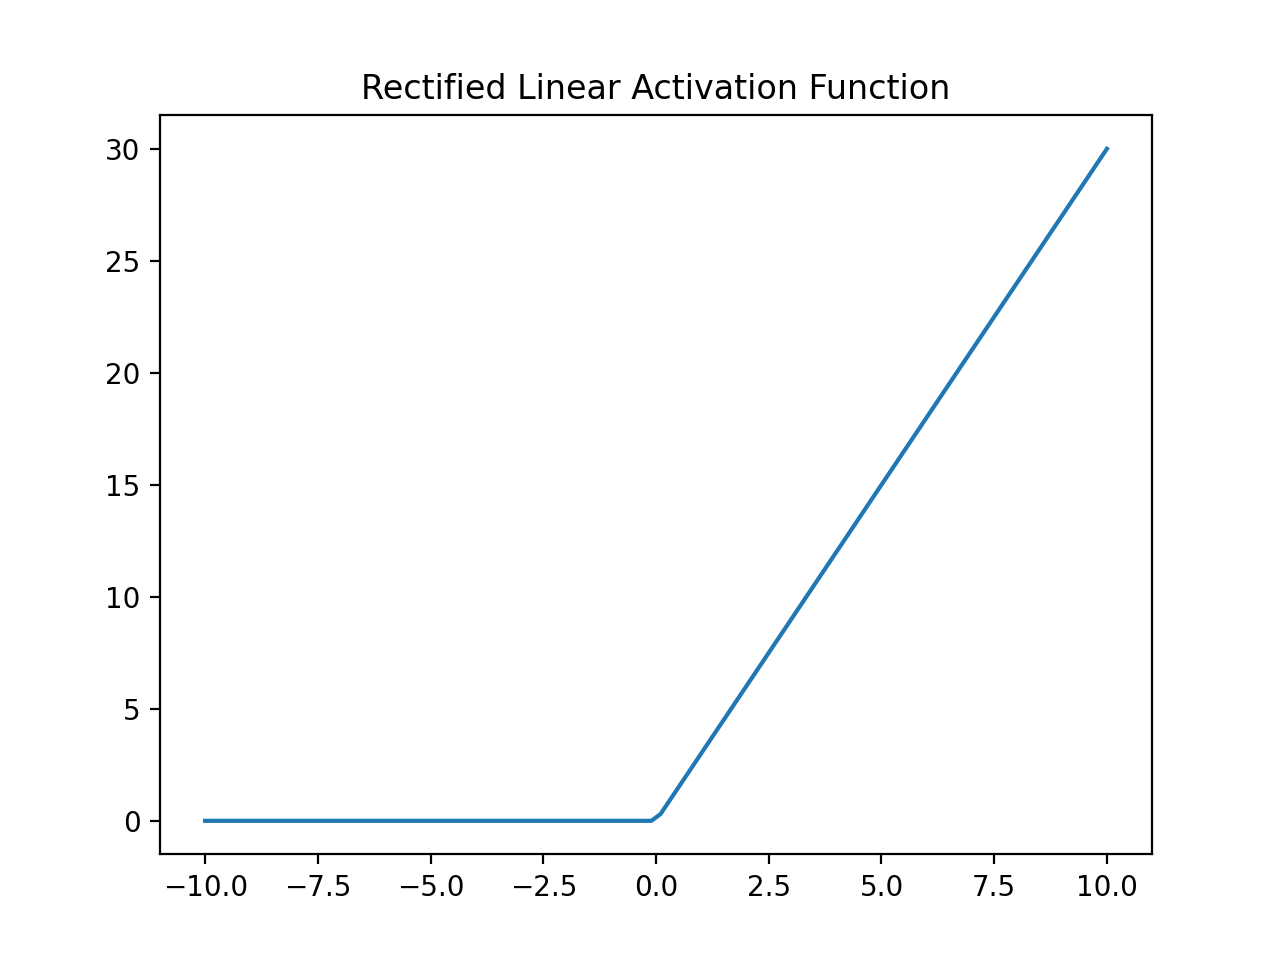
\includegraphics[width=.65\linewidth]{Images/relu.png}
    \caption{Sketch of the Rectified Linear Activation Function}
\end{figure}

Second, it outputs the results. Third, it compares the prediction to the ground truth using a loss function.

\begin{definition}
A loss function outputs an error value which is an estimate of how poorly the network is performing.
\end{definition}

The lost function that will be utilised in the software will be the function for mean squared error. The reason for choosing this particular function is that it heavily penalises large errors, as it squares the difference between the predicted and actual value. A large error in a weather forecast is highly undesirable, hence, the use of this function. The function is represented below:

\begin{equation}
    MSE = \frac{1}{n}\sum_{i=1}^n(Y_i-\hat{Y_i})^2
\end{equation}

If  a vector of $n$ predictions is generated from a sample of $n$ data points on all variables, and $Y$ is the vector of observed values of the variable being predicted, with $\hat{Y_i}$ being the predicted values.

\begin{definition}
Mean squared error is the average squared difference between the estimated values and the actual value.
\end{definition}

Returning to the training of the RNN, it uses that error value from the loss function. to do back propagation which calculates the gradients for each time step in the network. The gradient is the value used to adjust the networks internal weights, allowing the network to learn. The bigger the gradient, the bigger the adjustments and vice versa. Here is where the problem lies. When doing back propagation, the gradient of the current time step is calculated with respect to the effects of the gradients, in the time step before it. So if the adjustments to the time step before it is small, then adjustments to the current time step will be even smaller.  The gradient values will exponentially shrink as it propagates through each time step. That causes gradients to exponentially shrink as it back propagates down. The earlier layers fail to do any learning as the internal weights are barely being adjusted due to extremely small gradients.

Because of vanishing gradients, the RNN doesn’t learn the long-range dependencies across time steps. So not being able to learn on earlier time steps causes the network to have a short-term memory. In order to combat this, a long short-term memory is used\cite{intro_rnn}.

\subsection{LSTM}
LSTM's were created as a solution to the short-term memory problem. They have internal mechanisms called gates that can regulate the flow of information. These gates can learn which data in a sequence is important to keep or throw away. By doing that, it can pass relevant information down the long chain of sequences to make predictions. For example, if you were interested in buying a particular product, you might read a review in order to determine if the purchase of the product is a good decision. When you read a review, your brain subconsciously only remembers important keywords. You pick up words like ``amazing", ``superb", or ``awful", you don't remember words such as "the", "as", or "because". This is what an LSTM does, it learns to keep only the relevant information to make predictions.

An LSTM has a similar control flow as a recurrent neural network. It processes data passing on information as it propagates forward. The differences are the operations within the LSTM’s cells. The core concept of LSTM’s are the cell state, and it’s various gates. The cell state is the method by which information is transferred down the sequence chain. The cell state, in theory, can carry relevant information throughout the processing of the sequence. So even information from the earlier time steps can make its way to later time steps, reducing the effects of short-term memory. As the cell state goes on its journey, information gets added or removed to the cell state via gates\cite{lstm_rnn}.

\begin{definition}
A gate is an electric circuit with an output which depends on the combination of several inputs.
\end{definition}

Gates contain the sigmoid activation function. The sigmoid activation function squishes values between 0 and 1. That is helpful to update or forget data because any number getting multiplied by 0 is 0, causing values to disappears or be ``forgotten". Any number multiplied by 1 is the same value therefore that value stay’s the same or is ``kept".

\begin{figure}[H]
    \centering
    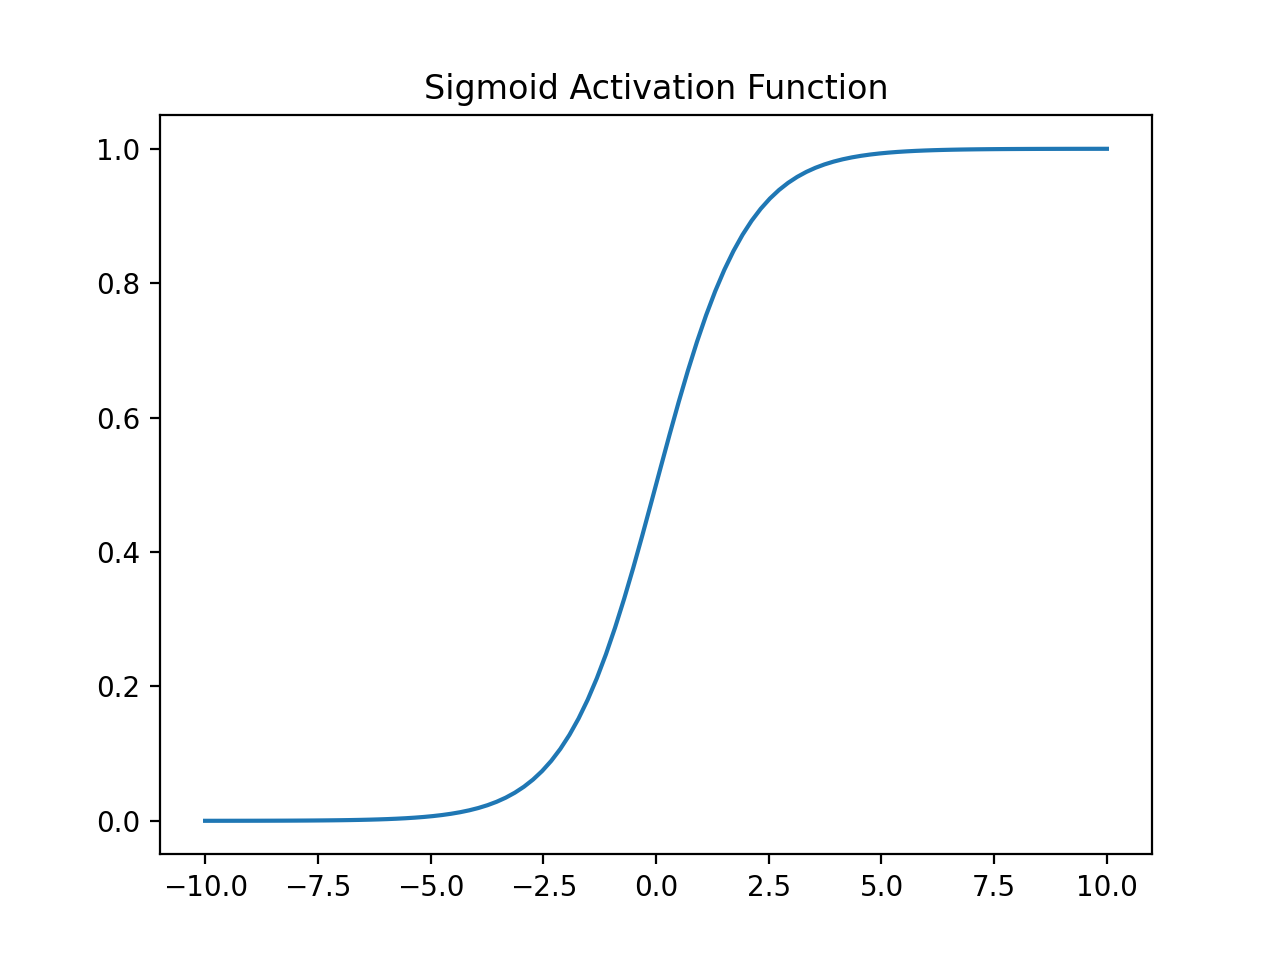
\includegraphics[width=.65\linewidth]{Images/sigmoid.png}
    \caption{Sketch of the Sigmoid Activation Function}
\end{figure}

There are three types of gates utilised within a neural network: a forget gate, an input gate, and an output gate. A forget gate decides what information should be thrown away or kept. Information from the previous hidden state and information from the current input is passed through the sigmoid function. An input gate is where the previous hidden state and current input are passed into a sigmoid function. The output gate decides what the next hidden state should be. The hidden state is also used for predictions. First, we pass the previous hidden state and the current input into a sigmoid function. Then we pass the newly modified cell state to the rectified linear activation function. We multiply the rectified linear activation function output with the sigmoid output to decide what information the hidden state should carry. The output is the hidden state. The new cell state and the new hidden is then carried over to the next time step\cite{lstm_rnn}.

\subsection{Principal Component Analysis}\label{pca_section}
The number of features in a dataset is referred to as its dimensionality. Dimensionality reduction refers to techniques that reduce the number of input variables in a dataset. More input features often make a predictive modelling task more challenging to model, and can be computational expensive. Considering dimensionality reduction is a data preparation technique performed on data prior to modelling, it might be performed after data cleaning and data scaling and before training a predictive model\cite{dimension_reduction}. 

For a given training window, there is 22,032,000 points. Attempting such a dataset would be computational burdensome, hence, the attractiveness of dimensionality reduction. Dimensionality reduction can reduce the number of data points without severely impacting accuracy. Fewer input dimensions often mean correspondingly fewer parameters or a simpler structure in the machine learning model, referred to as degrees of freedom. A model with too many degrees of freedom is likely to overfit the training dataset and therefore may not perform well on new data. It is desirable to have simple models that generalise well, and in turn, input data with few input variables. The problem is high-dimensional functions have the potential to be much more complicated than low-dimensional ones, and that those complications are harder to discern. The only way to beat this problem is to incorporate knowledge about the data that is correct\cite{dimension_reduction}. A popular choice for dimensionality reduction is principal component analysis, and was the technique selected for this project. 

\begin{definition}
Principal Component Analysis, is a dimensionality reduction method that is often used to reduce the dimensionality of large data sets, by transforming a large set of variables into a smaller one that still contains most of the information in the large set.
\end{definition}

Reducing the number of variables of a data set naturally comes at the expense of accuracy, but the trick in dimensionality reduction is to trade a little accuracy for simplicity. Because smaller data sets are easier to explore and visualise and make analysing data much easier and faster for machine learning algorithms without extraneous variables to process\cite{pca}. 

First, the dataset is standardised to the range of the continuous initial variables so that each one of them contributes equally to the analysis. Second, to see if there is any relationship between the variables of the input dataset, covariance matrix computation is done. The covariance matrix is not more than a table that summaries the correlations between all the possible pairs of variable. The eigenvectors and eigenvalues of the covariance matrix is computed in order to identify the principal components. Principal components are new variables that are constructed as linear combinations or mixtures of the initial variables. PCA tries to put maximum possible information in the first component, then maximum remaining information in the second and so on. Organizing information in principal components this way, will allow for the reduction of dimensionality without losing much information, and  by discarding the components with low information and considering the remaining components as your new variables\cite{pca}. For the purposes of this project, 99\% of the variance was retained in order to balance accuracy with reducing the number of features. 

\section{Dataset}
\subsection{ERA5 Atmospheric Reanalysis Dataset}\label{era5_dataset}
ERA5 provides hourly estimates of a large number of atmospheric, land and oceanic climate variables. The data covers the Earth on a 30km grid and resolves the atmosphere using 137 levels from the surface up to a height of 80km. ERA5 includes information about uncertainties for all variables at reduced spatial and temporal resolutions. Quality-assured monthly updates of ERA5 are published within 3 months of real time. Preliminary daily updates of the dataset are available to users within 5 days of real time. ERA5 combines vast amounts of historical observations into global estimates using advanced modelling and data assimilation systems\cite{era5}.

The ERA5 reanalysis dataset was used for training, validating and testing the performance of the neural network architecture. Reanalysis datasets provide the best guess of the atmospheric state at any point in time by combining a forecast model with the available observations. The raw data is available hourly for 40 years from 1979 to 2019 on a $0.25^{\circ}$ latitude-longitude grid ($721 \times 1440$ grid points) with 37 vertical levels. Since this raw dataset is quite significant, it is necessary to regrid the dataset to a lower resolution and use a smaller fraction of the available dataset\cite{rasp2020weatherbench}.  The poles were excluded from the dataset in order to avoid a singularity, and the potential negative impact that could have on predictive ability of the neural network.

It was ultimately decided to use a spatial resolution of $3^{\circ}$ ($60 \times 120$ grid points) and a temporal resolution of 2 hours. In regards to pressure surfaces, 17 vertical pressure levels were ultimately chosen:  1, 2, 5, 10, 20, 50, 100, 200, 300, 400, 500, 600, 700, 800, 900,  950, 1000 hPa. Note that it is common to use pressure in hectopascals as a vertical coordinate instead of physical height. The pressure at sea level is approximately 1000 hPa and decreases roughly exponentially with height. 850 hPa is at around 1.5 km height. 500 hPa is at around 5.5 km height. The data is split into yearly NetCDF files for each variable. The entire dataset at $3^{\circ}$ resolution has a size of 75GB. The available variables were chosen based on meteorological consideration. Geopotential, temperature, humidity and wind are prognostic state variables in most physical NWP and climate models\cite{rasp2020weatherbench}. 

\subsection{Integrated Forecasting System}\label{ifs_section}
The Integrated Forecast System is a global numerical weather prediction system jointly developed and maintained by the European Centre for Medium-Range Weather Forecasts. The version of the IFS run at ECMWF is often referred to as the "ECMWF" or the "European model" in North America, to distinguish it from the American GFS. It comprises a spectral atmospheric model with a terrain-following vertical coordinate system coupled to a 4D variational data assimilation system. In 1997 the IFS became the first operational forecasting system to use a 4D variational, data assimilation system

\begin{definition}
4D dimensional variational data assimilation system adjusts a short-range forecast, called the background, in space and time to bring it into closer agreement with meteorological observations.
\end{definition}

It is one of the predominant global medium-range models in general use worldwide; its most prominent rival is in the 6–10 day medium range include the American Global Forecast System, the Canadian Global Environmental Multiscale Model and the UK Met Office Unified Model. It is the gold standard of medium-range numerical weather prediction. The current IFS deterministic forecast is computed on a cluster with 11,664 cores. One 10 day forecast at 10 km resolution takes around 1 hour of real time to compute\cite{rasp2020weatherbench}. The Integrated Forecasting System will be used as a comparison against the neural network.

\begin{figure}[H]
    \centering
    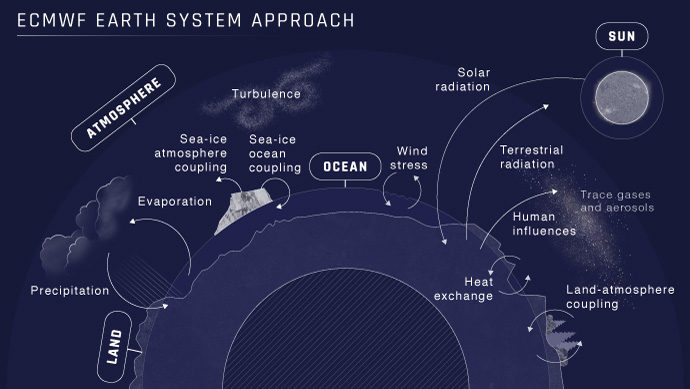
\includegraphics[width=.8\linewidth]{Images/ifs.jpg}
    \caption{ECMWF Integrated Forecast System}
\end{figure}

To provide physical baselines more in line with the current resolution of the neural network, it was compared against the IFS model at two coarser horizontal resolutions, T42 (approximately $2.8^{\circ}$) with 62 vertical levels and T63 (approximately $1.9^{\circ}$) with 137 vertical levels. It must be noted that I personally did not generate such forecasts, or perform the analysis on said forecasts. It acquired the results from Weather Bench, a benchmark dataset for data-driven weather forecasting. According to said source; computationally, a single forecast takes 270 seconds for the T42 model and 503 seconds for the T64 model on a single XC40 node with 36 cores.

\section{Implementation}\label{implement_rnn}
The dataset consists of five features: geopotential, zonal wind, meridional wind, air temperature, and relative humidity. For a single day, there will be twelve observations. The goal for this project will be to predict the relevant atmospheric parameter in 6 hours time given the last fifteen days of data. In order to make such predictions, it is necessary to create a window of the last 180 ($15 \times 12$) observations to train the model\cite{time_series}. The neural network was trained on observational data from 2005 to 2016. The remainder of the dataset, 2017 to 2019, was preserved for validation, testing and benchmarking the neural network against physics-based models.

At the start, a seed is set in order to ensure reproducibility. As mentioned previously, it is important to scale features before training a neural network. Normalisation is a common way of doing this scaling by subtracting the mean and dividing by the standard deviation of each feature. In order for the most optimal performance, the method ``MinMaxScaler" from the library, scikit-learn, is utilised within the software\cite{scikit-learn}. An LSTM requires a 1-dimensional sequence, however, the atmosphere is a 3-dimensional system. Hence, it is necessary to flatten the 3-dimensional vector that represents the state of the atmosphere. This is done in order to avoid the need of repeatably running the RNN. Batches are then created to split the data into manageable sequences. A large batch size is used in order to greater emphasise values at the extremes, as such observations are particularly important in numerical weather predictions in tracking hurricanes and tornadoes. The diagram on the following page shows how the data is represented after flattening the data and batching it (provided by Tensorflow)\cite{time_series}.

\begin{figure}[H]
    \centering
    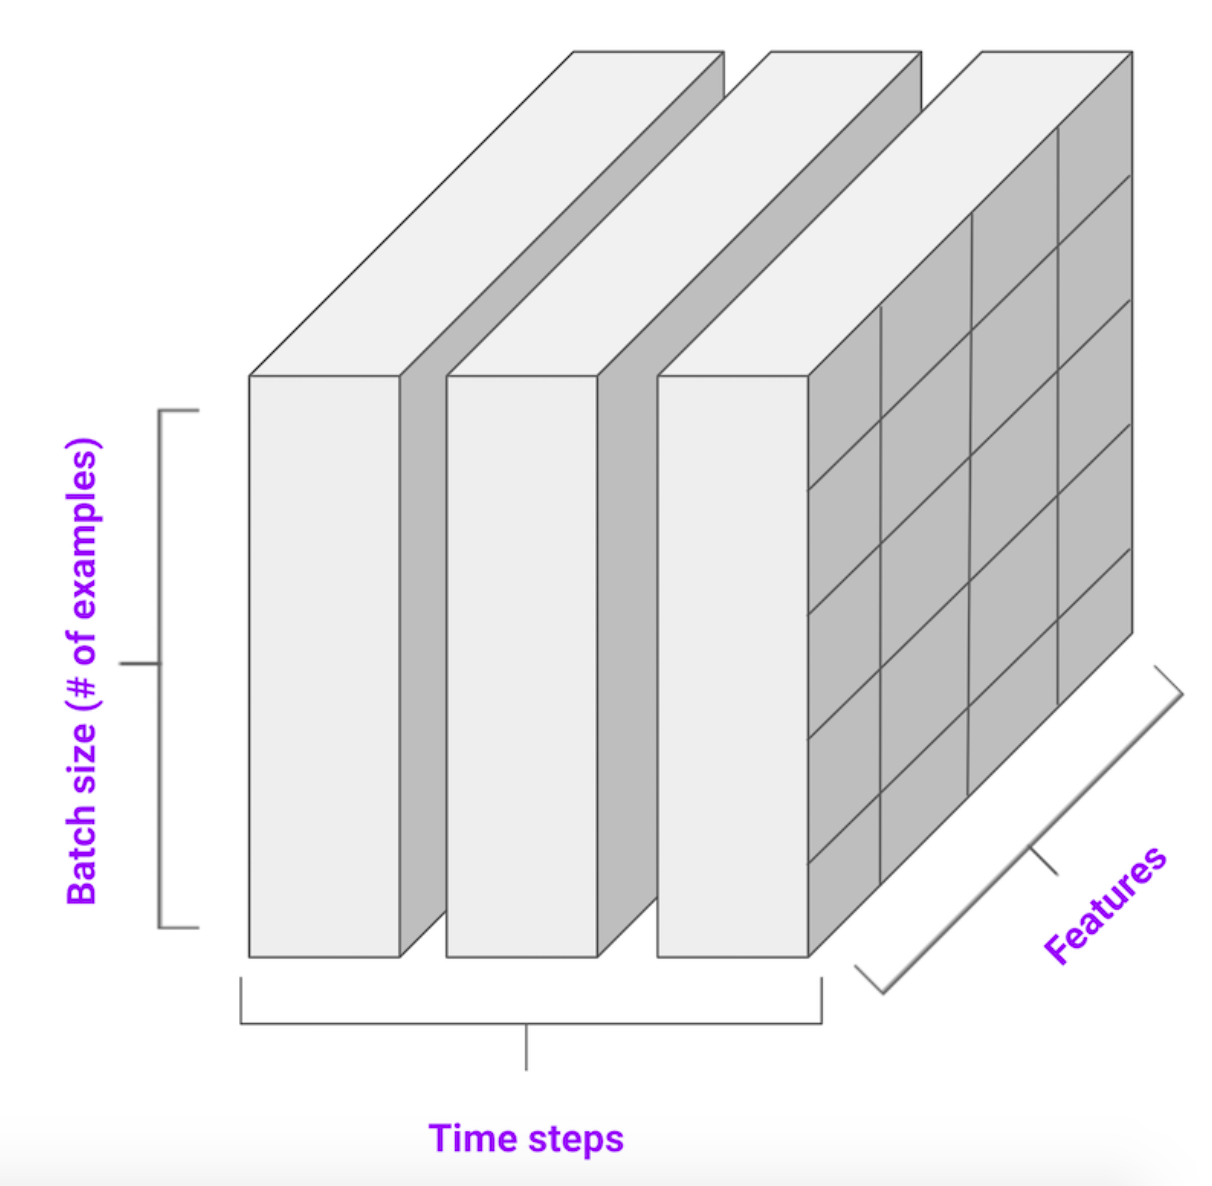
\includegraphics[width=.5\linewidth]{Images/data_rnn.png}
    \caption{Visualisation of how the data is represented after flattening and batching.}
\end{figure}

Following this process, the data is fed into the RNN. The LSTM model is built using Keras in TensorFlow, which is an free and open-source software library for machine learning. It was developed by the Google Brain Team\cite{tensorflow}. It is apparent that a multi-step model is needed as the model needs to learn to predict a range of future values. The source code for the LSTM model developed for the software is shown below:

\begin{minted}[mathescape,linenos,frame=lines]{python}
# Prepossessed historical data, which has been flatten and batched.
x_data, y_data, x_val, y_val = prepossessing_function(input_data)
# Prepossessed initial conditions, which has been flatten and batched.
initial_conditions = prepossessing_function(input_initialconditions)

# The network is shown data from the last 15 days.
past_history = 15 * 12

# The network predicts the next 6 hours worth of steps.
future_target = 0.5 * 12

# Create, and train models.
# Optimiser.
opt = Adam(lr=1e-3, decay=1e-5)
# Create model.
model = Sequential()
model.add(
    LSTM(
        480, activation='relu', input_shape=(past_history, features)
    )
)
model.add(RepeatVector(future_target))
model.add(LSTM(480, activation='relu', return_sequences=True))
model.add(TimeDistributed(Dense(features)))
model.compile(
    optimizer=opt, loss='mse', metrics=['mean_absolute_error']
)

# Train.
model.fit(
    x_data, y_data, validation=(x_val, y_val), epochs=epochs, batch_size=120
)

# Predict (this function is iterated to the forecast length required).
future_state = model.predict(initial_conditions)
# Invert normalisation, and flattening.
future_state = inverse_prepossessing(future_state)
\end{minted}

The model consists of four LSTM layers, which in combination are able to produce a more accurate and reliable prediction than a single LSTM layer. As is evident, the activation function for each LSTM is the rectified linear activation function, which is built into Keras. The number of epochs can be specified by the end user depending on the computational resources they have and what they need. More epochs will evidently lead to a more accurate neural network.

\begin{definition}
An epoch is one forward pass and one backward pass of all the training examples.
\end{definition}
